%%%%%%%%%%%%%
% Lecture 1 %
%%%%%%%%%%%%%


In this section, we introduce the concept of path integrals in the context of \emph{Markovian stochastic processes.}
Stochastic processes, such as a pollen particle in water affected by the random thermal fluctuations of the liquid particles bumping into it, are described by probability distributions.
\emph{Conditional} probabilities are statements of the form ``Given this initial state, what is the probability that the system ends up in that final state?'', and are therefore a function of all possible ways the system can evolve between these states.
We can therefore describe conditional probabilities of a physical process as a weighted sum (actually, an integral) of all possible ``paths'' the system can take between its initial and final state.


\section{Stochastic processes}

A stochastic process $x(t)$ is a sequence of random variables, indexed by $t \in \Te$.
The variable $t$ can be either discrete or continuous, the only requirement on $\Te$ being that it is \emph{totally ordered}.
Roughly, this means that, for any two elements $t_1, t_2 \in \Te$ and $t_1 \neq t_2$, then $t_1 < t_2$ or $t_2 < t_1$.
The most common example of $\Te$ is time, so $x(t)$ describes the evolution of $x$ thought time.
However, $\Te$ might also be the set of indices of monomers in a linear polymer chain, or of symbols printed on a thin paper strip, to give a couple of examples.
We will begin by considering discrete time steps with a length of $\Delta t$, so
%
\begin{align}
    \Te = \{ \dots -2 \Delta t, - \Delta t, 0, \Delta t, 2 \Delta t, \dots\} = \Delta t \Z.
\end{align}
%
The notation $\Delta t \Z$ means set of all integers $\Z$ multiplied by $\Delta t$.

We begin by considering a one-dimensional process, so $x \in \Ex$ is a scalar, but it may be either discrete or continuous.
A discrete process, with for example $\Ex = \Delta x \Z$, can be though of as a particle on a one-dimensional lattice with lattice points separated by $\Delta x$.
The probability that, if the particle is at lattice point $x = n \Delta x$ at time $t$, it will jump to lattice point $x' = m \Delta x$ at the next time step $t + \Delta t$, is denoted by $P\left(x'(t + \Delta t) | x(t) \right)$.
This is illustrated in \autoref{fig: stochastic process}.
We use there the common notation for conditional probabilities, where $P(A|B)$ means ``the probability of $A$ given $B$''.
It is defined as 
%
\begin{align}\label{eq: cond prob}
    P(A|B) P(B) = P(A\cap B),
\end{align}
%
where $P(A\cap B)$ is the probability that \emph{both} $A$ and $B$ occur.


\begin{figure}[!htb]
    \centering
    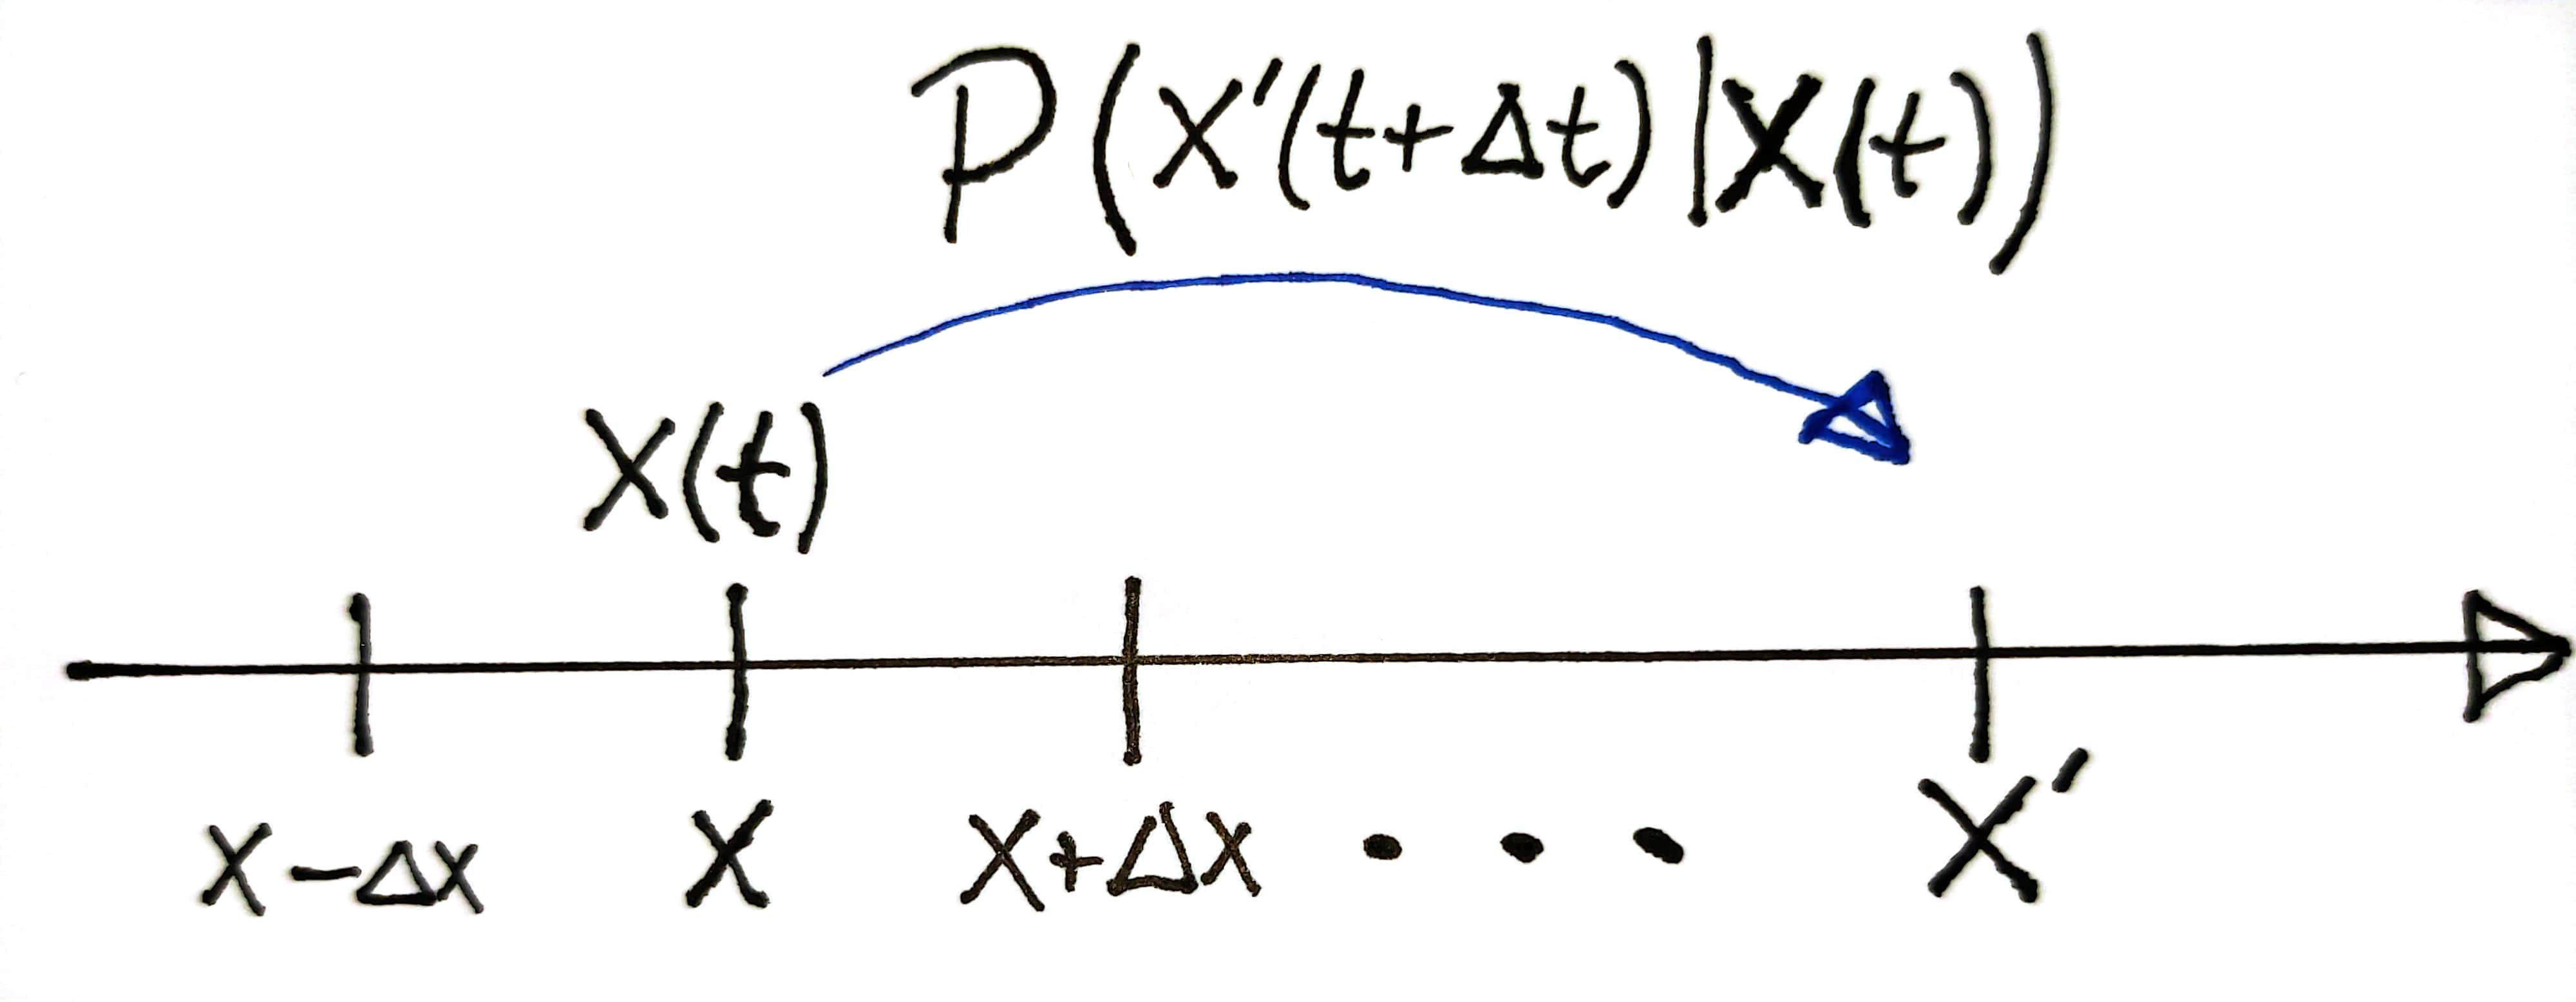
\includegraphics[width=.4\textwidth]{fig/fig1.jpg}
    \caption{Illustration of a stochastic process}
    \label{fig: stochastic process}
\end{figure}


A \emph{Markov process} is a stochastic process with ``no memory''.
This means that, if we have $n$ steps of the process, denoted $x(t_1), x(t_2), \dots x(t_n)$, then the conditional probability of observing $x(t_n)$ given $x(t_1), \dots x(t_{n-1})$, only depends on the last step $x(t_{n-1})$.
This can be stated as
%
\begin{align}
    P(x_n |x_{n-1}, x_{n-2}, \cdots, x_1) = P(x_n | x_{n-1}).
\end{align}
%
Here, we use the shorthand $x_i = x(t_i)$.

As far as we know, the underlying laws of physics are fully described at each time-step, so the question of whether we can model a process as Markovian depends on our description.
For example, if try to describe the flight of a football through the air with only its position, the description is not Markovian, as we need the current velocity to know where it will be at the next time-step.
But, if we include the velocity in our description, the model is Markovian.
A non-Markovian description thus indicate that we have excluded degrees of freedom that contain information about the system.
Be aware that a system being Markovian does not imply statistical independence, so $P(x_{n}, x_{n-1})\neq P(x_n)P(x_{n-1})$


From the definition of conditional probability, \autoref{eq: cond prob}, we can derive that the joint probability of three sequential events, $x_1$, $x_2$ and $x_3$ is given by
%
\begin{align}
    P(x_1, x_2, x_3) = P(x_3|x_2,x_1)P(x_2|x_1)P(x_1).
\end{align}
%
A Markovian process thus has the property
%
\begin{align}
    P(x_1, x_2, x_3) = P(x_3|x_2)P(x_2|x_1)P(x_1).
\end{align}
%
We can furthermore write $P(x_3, x_1) = \sum_{x_2 \in \Ex} P(x_3, x_2, x_1)$.
From this, we derive the Chapman-Kolmogorov equation,
%
\begin{align}\label{eq: chapman kolmogorov}
    P(x_3|x_1) = \sum_{x_2} P(x_3|x_2) P(x_2|x_1).
\end{align}
%
By repeatedly applying this process, we can get conditional probability between two steps $x_1$ and $x_{n+1}$ arbitrarily far removed,
%
\begin{align}\label{eq: cond prob markov x0 given xn}
    P(x_{n+1}|x_1) 
    = \sum_{ x_2, \dots x_n}
    P(x_{n+1}|x_n) P(x_n| x_{n-1})\dots P(x_2|x_1).
\end{align}
%
We see that this already begins to resemble something like a sum over all possible ``paths'' that the proces $x(t)$ can take to transition from $x_1$ at $t_1$ to $x_{n+1}$ at $x(t_{n+1})$.
This is illustrated in \autoref{fig: paths}.


\begin{figure}[!htb]
    \centering
    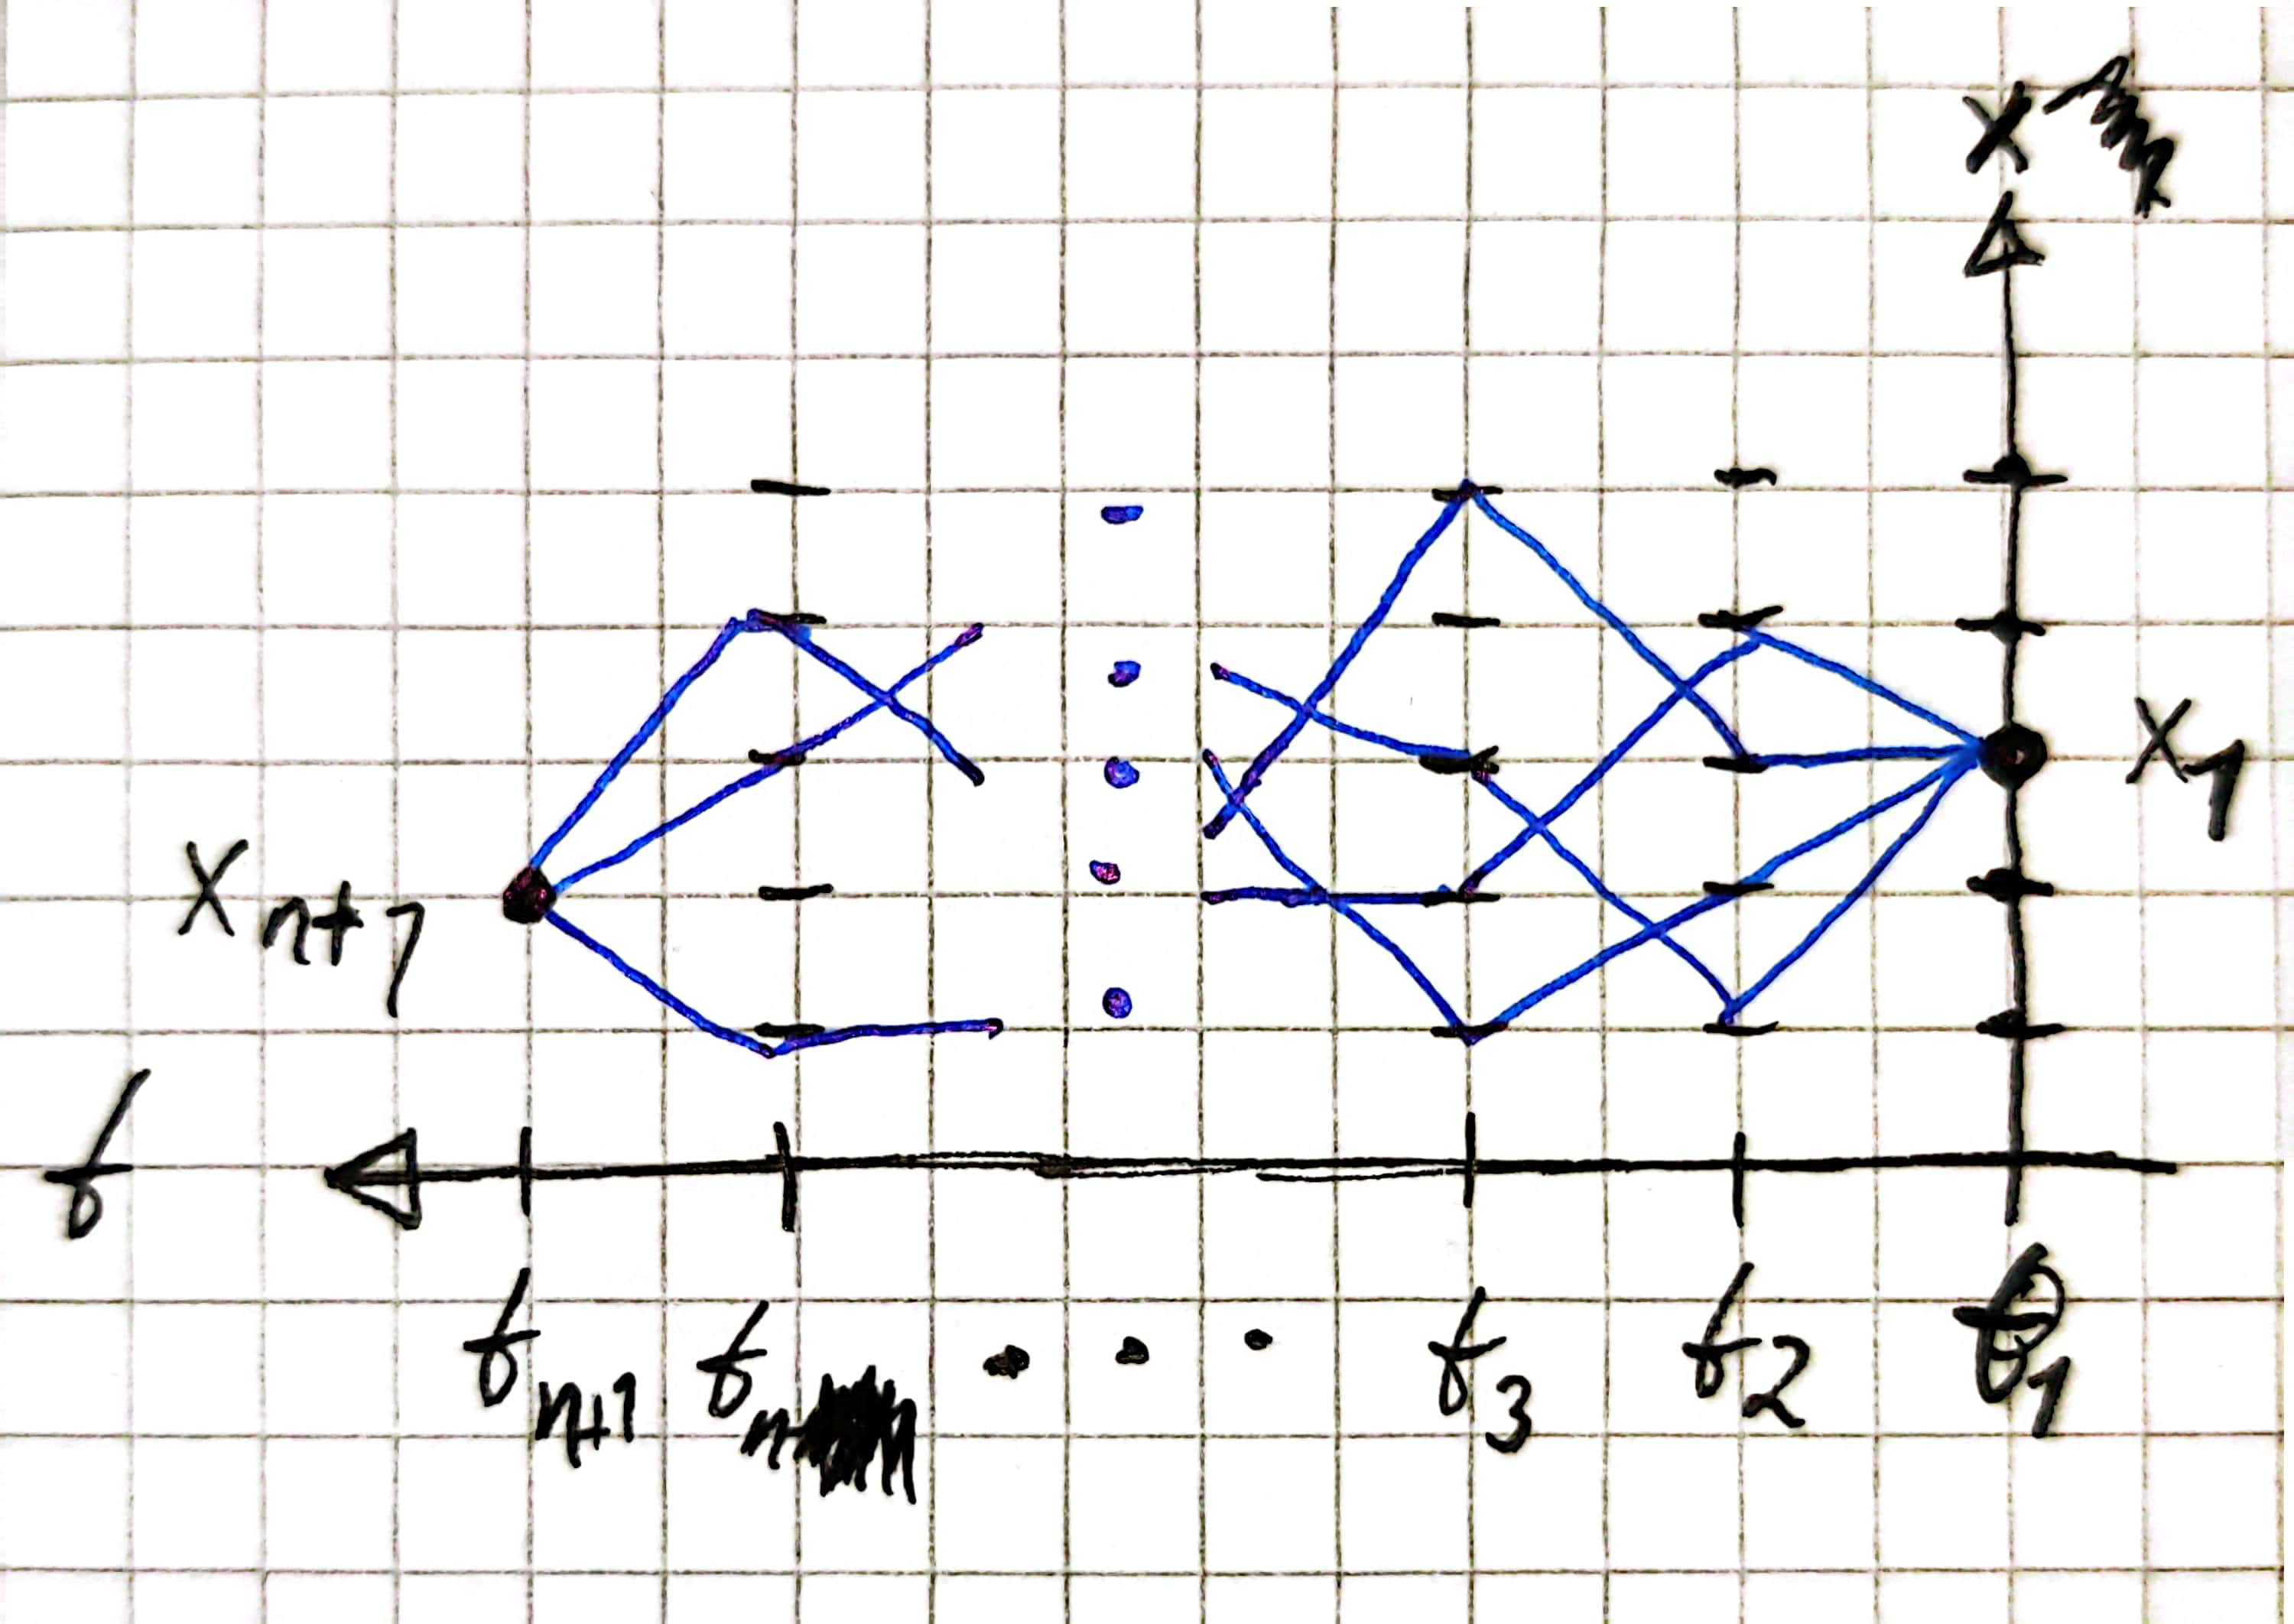
\includegraphics[width=.4\textwidth]{fig/fig2.jpg}
    \caption{Some of the paths between the initial and final state.}
    \label{fig: paths}
\end{figure}


\subsection*{The continuum limit}
\label{subsection: continuum limit}

If we consider a particle on a line instead of a lattice, so $\Ex = \R$, we must consider \emph{probability densities} $\Pe(x)$.
The probability of finding the particle between the points $x_i$ and $x_i + \Delta x$ is, for small $\Delta x$,
%
\begin{align}\label{eq: probability density}
    P(x) \equiv P(x \in [x_i, x_i + \Delta x]) = \Delta x \Pe(x).
\end{align}
%
This corresponds to the limit $\Delta x \rightarrow 0$ for the discrete process considered above, and allows us to go from sums to integrals,
%
\begin{align}
    \sum_{x} P(x) \sim \sum_{x} \Delta x \Pe(x) \underset{\Delta x \rightarrow 0}{\longrightarrow} \int \dd x \, \Pe(x).
\end{align}
%
In this limit the Chapman-Kolgomorov equation, \autoref{eq: chapman kolmogorov}, becomes
%
\begin{align}\label{eq: chapman kolgomorov cont}
    \Pe(x'|x) = \int \dd x'' \, \Pe(x'|x'') \Pe(x''|x),
\end{align}
%
and \autoref{eq: cond prob markov x0 given xn} becomes
%
\begin{align}\label{eq: cond prob markov x0 given xn cont}
    P(x_{n+1}|x_1) 
    = \left(\int \prod_{i=2}^{n} \dd x_i\right)
    \Pe(x_{n+1}|x_n) \Pe(x_n| x_{n-1})\cdots \Pe(x_2|x_1).
\end{align}

Likewise, we can take the limit $\Delta t\rightarrow 0$, corresponding to $n\rightarrow\infty$, to obtain a process with continuous time.
In this case (the ``continuum limit'') \autoref{eq: cond prob markov x0 given xn cont} becomes
%
\begin{align}\label{eq: general path integral}
    P(x(t_0 + T) | x(t_0) ) 
    &
    =
    \lim_{
        \substack{\Delta x \rightarrow 0\\n\rightarrow \infty}
    }
    \left(\int \prod_{i = 1}^{n} \dd x_i C_n\right)
    \Phi_n(\{x_i\})
    \equiv
    \int \D x(t) \, \Phi[x(t)].
\end{align}
%
where $\Delta t = T/n$ and $t_i = t_1 + (i-1)\Delta t$.
We have defined 
%
\begin{align}
    \Phi(\{x_i\}) = \frac{1}{C_n} \Pe(x(t_{n+1}) | x(t_n) ) \cdots \frac{1}{C_n} \Pe(x(t_{2}) | x(t_1) ),
\end{align}
%
where $C_n$ is a constant we will come back to later.
In the last equality, we have defined the \emph{path integral measure} $\D x(t) = \lim_{n \rightarrow \infty} \prod_{i=1}^n \dd x(t_i) C_n$,
and the \emph{functional} $\Phi[x(t)]= \lim_{n \rightarrow \infty} \Phi_n(\{x_i\})$ emerging from the infinite product of conditional probabilities.
This is a functional and not a function, as it itself takes as its argument a function $x(t)$ and returns a number.
We see that \autoref{eq: general path integral} gives the conditional probability for $x(t_0 + T)$ given $x(t_0)$ by integrating over all possible paths $x(t)$ weighted by $\Phi[x(t)]$.
For now, this is a very formal quantity.
To see the power of this formalism, we consider a concrete process, the Ornstein-Uhleneck process.



\section{Gaussian processes and the Ornstein-Uhlenbeck process}
\label{sectoin: gaussian and OUP}

The most important class of stochastic processes, as it is pretty much the only one we can solve, is Gaussian processes, which are processes with probability densities with the form
%
\begin{align}
    \Pe(x_{n+1}|x_n)
    =
    \frac{ 1 }{ \sqrt{ 2 \pi \sigma_{n+1} } }
    \exp \left\{ {-\frac{(x_{n+1} - \bar x_{n + 1})^2}{2 \sigma_{n+1} }} \right\}
\end{align}
%
Here, $\bar x_{n+1}$ is the expected value of $x_{n+1}$, and $\sigma_{n+1}$ the variance.
As we consider Markovian processes, these quantities are functions of (equivalently, conditioned on) only the previous step, $x_n$.


If we have a vector valued process instead, $\bm x(t) = x_a(t) \hat {\bm x}_a$, then the probability distribution is a multivariate Gaussian
%
\begin{align}
    P(x_{n_1}|x_n)
    = 
    \frac{ 1 }{ \sqrt{ 2 \pi \det \Sigma } }
    \exp \left\{ - \frac{1}{2}\sum_{ab} \left[x_a(t_{n+1}) - \bar x_a(t_{n+1})\right] \Sigma_{ab}^{-1} \left[x_b(t_{n+1}) - \bar x_b(t_{n+1})\right] \right\}.
\end{align}
%
Here, $\Sigma$ is the covariance matrix of $x$.
An example of this may be a particle moving in three dimensions, so $\bm x$ is a three-dimensional vector, or a set of $N$ particles with position and velocity in three dimensions, so $\bm x$ is a $6 N$ component vector.


A specific example is the Ornstein-Uhlenbeck (OU) process, which in one dimension is
%
\begin{align}\label{eq: OUP}
    \odv{ x(t) }{ t } = - \mu x(t) + \eta(t).
\end{align}
%
This models, for example, a particle on a spring in a fluid with thermal noise where friction dominates and inertial effects are negligible.
The linear restoring term $-\mu x(t)$ is from Hooks law, and $\eta(t)$ is a zero-mean random force modeling the forces of the fluid particles bumping into the particle.
You can read more about this process in~\footnote{\url{https://iopscience.iop.org/article/10.1088/1367-2630/ad7ef1/meta}}.
For small $\Delta t$, the expectation value of the OU-process at time $t_{n+1}$ conditioned on $x(t_n)=x_n$ is $\bar{x}_{n+1} = x_n - \mu x_n \Delta t$ --- i.e. where it was the step before minus the correction due to the spring-force.
The variance is $\sigma_{n+1} = 2D \Delta t$, where $D$ is the diffusion constant, which is the variance of the noise $\eta$. Note that this latter quantity does not depend on $x_n$.
With this, OU-process has the conditional probability density for small $\Delta t$
%
\begin{align}
    \Pe(x_{n + 1}| x_n) 
    = \sqrt{ \frac{ \mu }{ 4 \pi D \Delta t } }
    \exp \left\{ -
    \frac{ \left(x_{n + 1} - x_n + \mu x_n \Delta t\right)^2 }{ 4 D \Delta t } 
    \right\}
    = \sqrt{ \frac{ \mu }{ 4 \pi D \Delta t } }
    \exp \left\{ 
    - \frac{ \Delta t }{ 4 D }  \left(\dot x_{n + 1} + \mu x_n\right)^2
    \right\},
\end{align}
%
where we have introduced the discrete time-derivative, $\dot x_{n+1} = (x_{n + 1} - x_n) / \Delta t$.
In the $\Delta t \rightarrow 0$ limit, this becomes a regular derivative.



Inserting the OU process into \autoref{eq: cond prob markov x0 given xn} and taking the continuum limit as discussed above, we get
%
\begin{align}\label{eq:om_func}
    P(x_{n+1}|x_{1})
    & =
    \sum_{x_2\cdots x_{n+1}}
    \Delta x \Pe \left( x_{n+1}| x_{n} \right) \cdots \Delta x \Pe \left( x_{2}| x_{1} \right)\\
    &
    = \sum_{x_2\cdots x_{n+1}} \Delta x^n \exp \left\{ - \frac{\Delta t}{4 D} \sum_n \left[\dot x_{n + 1} - \mu x_n \right]^2 \right\}\\
    & 
    \underset{\substack{\Delta x \rightarrow 0\\ n \rightarrow \infty} }{ \sim }
    \int \D x(t) \,
    \exp \left\{ 
        - \frac{ 1 }{ 4D } 
        \int\limits_{t_1}^{t_{n+1}} \dd t \left[\dot x(t) + \mu x(t)\right]^2
        \right\}
    \equiv
    \int \D x(t) \, \Phi[x(t)].
\end{align}
%
In this case, the integration measure is
%
\begin{align}
    \D x(t) \equiv \lim_{\substack{\Delta x \rightarrow 0\\ n \rightarrow \infty} } \prod_{n} \Delta x \sqrt{ \frac{\mu}{ 4 \pi D \Delta t }},
\end{align}
%
which corresponds to $C_n = \sqrt{\mu/4\pi D \Delta t}$.
This measure is not strictly well-defined. 
To performed calculations, we will have re-descritize the path integral, so this can be considered as a notational trick rather than a true limit. The functional $\Phi[x(t)]$ in Eq.~\eqref{eq:om_func} is often referred to as the Onsager-Machlup functional, thanks to its appearance in a 1953 paper by the two physicists. We'll come back to it later on in the course.


\section{Master equation}

We will here consider stochastic processes using a different formalism, the master equation. While this formalism will be relevant later on in the course, we introduce it early on to make a point about the equivalence between the path integral representation of stochastic process and other, more common approaches.
If we consider a discrete stochastic process $N(t)$, and Taylor-expand the conditional probability of $N'$ at $t + \Delta t$ given $N$ at $t$ in small $\Delta t$, we get
%
\begin{align}\label{eq: expansion cond prob}
    P(N'(t + \Delta t)| N(t)) = 
    \underbrace{P(N'(t)|N(t))}_{\delta_{N'N}} + \Delta t 
    \underbrace{\pdv{P(N'(t')|N(t))}{t'}\bigg|_{t'=t}}_{W_t(N'|N)} + \Oh(\Delta t).
\end{align}
%
Here, we define the \emph{transition rates} $W_t(N'|N)$. The subscript highlights the fact that these may explicitly depend on time: for example, if the stochastic process $N(t)$ describes the number of individuals in the population of a particular species of insects, the transition rates $W_t(N+1|N)$ and $W_t(N-1|N)$ associated with birth and death processes might depend explicitly on time through seasonal variations in temperature.

The transition rate $W_t(N'|N)$ can be considered as a matrix, 
%
\begin{align}
    W_t(N'|N) = 
    \begin{pmatrix}
        W_t(1|1) & W_t(1|2)& W_t(1|3) &\cdots\\
        W_t(2|1) & W_t(2|2)& W_t(2|3) &\cdots \\
        \vdots & \vdots & \ddots & \cdots
    \end{pmatrix},
\end{align}
%
where the entries are the rate at which state $N$ transitions to state $N'$.
If we consider $N' = N$, then we can, by the principle of total probability (the probability of all possible outcomes add up to one), write
%
\begin{align}
    P(N(t + \Delta t)| N(t)) = 1 + \Delta t W_t(N|N) 
    = 1 - \sum_{N' \neq N}P(N'(t + \Delta t)| N(t))
    = 1 - \sum_{N' \neq N}\Delta t W_t(N',N),
\end{align}
%
or equivalently
%
\begin{align}\label{eq: rate cons condition}
    W_t(N|N) = - \sum_{N'\neq N}W_t(N'|N).
\end{align}
%
This insures the conservation of probability.
If we consider the matrix form of the rates, this means the diagonals of $W_t(N'|N)$ are given by minus the sum of the off-diagonal elements in each column,
%
\begin{align}
    W_t(N'|N) = 
    \begin{pmatrix}
        - \sum_{N\neq 1} W_t(N|1) & W_t(1|2)& W_t(1|3) &\cdots\\
        W_t(2|1) & - \sum_{N\neq 2} W_t(N|2)& W_t(2|3) &\cdots \\
        \vdots & \vdots & \ddots & \cdots
    \end{pmatrix},
\end{align}
%
If we expand the Chapman-Kolmogorov, \autoref{eq: chapman kolmogorov},
%
\begin{align}
    P(N(t_3) |N(t_1))
    & =
    \sum_{N(t_2)} 
    \left[
        \delta_{N(t_3)N(t_2)}
        + (t_3 - t_2) W_{t_2}(N(t_3)|N(t_2))
    \right]
    P(N(t_2)|N(t_1))
    \\
    & =
    (t_3 - t_2)\sum_{N(t_2)\neq N(t_3)} 
        W_{t_2}(N(t_3)|N(t_2)) P(N(t_2)|N(t_1))\\
    & \quad 
    + \left[ 1 + (t_3 - t_2) W_{t_2}(N(t_3)|N(t_2)=N(t_3))  \right] P(N(t_2)=N(t_3)|N(t_1))
\end{align}
%
If we apply \autoref{eq: rate cons condition}, and define $\Delta t = t_3 - t_2$, we can rearrange this to read
%
\begin{align}
    &\frac{P\left(N(t_3)|N(t_1)\right) - P(N(t_2)=N(t_3)|N(t_1))}{\Delta t}\\
    &=
    \sum_{N(t_2) \neq N(t_3)}
    \left[
        W_{t_2}(N(t_3)|N(t_2))P(N(t_2)|N(t_1))
        - W_{t_2}(N(t_2)|N(t_2)=N(t_3))P(N(t_2)=N(t_3)|N(t_1))
    \right]
\end{align}
%
The top line of this equation is the difference in probability of finding the system in the state $N(t_3)$ at time $t_3$ and $N(t_2)$, so in the limit $\Delta t \rightarrow 0$ becomes a derivative.
On the bottom, we have the difference between the \emph{gain} rate and the \emph{loss} rate in to and out of state $N(t_3)$
We take the limit, which gives the \emph{master equation},
%
\begin{align}
    \odv{}{t} P(N(t)|N_0) =
    \sum_{N'\neq N} \left[
        W_t(N(t)|N'(t))P(N'(t)|N_0)
        - 
        W_t(N'(t)|N(t))P(N(t)|N_0)
    \right].
\end{align}
%
Solving for $P(N(t)|N_0)$ by integrating the master equation will of course give the same result as computing the conditional probability by means of the corresponding path integral, since both are directly derived from the definition of the conditional probability distribution only by assuming the process is Markovian.
Although the two formulations are equivalent, they may be better or worse suited for different problems.

\begin{framed}
    \noindent
    \textbf{The quantum-stochastic analogy}\\
    The master equation is a first-order linear ODE giving the time-evolution of a probability distribution.
    If this reminds you of the Schrödinger equation for the quantum mechanical wave function, the similarities does not stop here.
    In fact, the correspondence between the master equation and the Onsager-Machlup functional is analogous to the relationship between the Schrödinger and the Feynman path integral in QM. Let's briefly revisit the latter.
    The classical action of a process is a functional
    %
    \begin{align}
        S[x] = \int\limits_{t_a}^{t_b} \dd t \, L(x, \dot x, t), 
    \end{align}
    %
    where $L = V - T$ is the Lagrangian.
    In classical mechanics, the motion is determined by the Euler-Lagrange equations, $\fdv{ S }{ x(t) } = 0$, while in quantum-mechaics, the amplitude for a process is, according to the Feynman path integral,
    %
    \begin{align}
        K(x_b | x_a) &= \sum_{\mathrm{paths}\, x} \Phi[x], & \Phi[x] \propto e^{iS[x] / \hbar}~.
    \end{align}
    %
    The Schrödinger equation gives the equivalent evolution of the wave-function,
    %
    \begin{align}
        i \hbar \odv{  }{ t } \Psi(x(t)) = \hat H \Psi(x(t)),
    \end{align}
    %
    where $\hat H$ is the Hamiltonian operator, and the amplitude is the overlap between the initial and finite wave-functions, $K(x_b | x_a) = \braket{ \Psi(x(t_b)) | \Psi(x(t_a)) } $. Just like the master equation can be derived from the Chapman-Kolmogorov equation, so can the Schrödinger equation be derived from the Feynman path integral representation of the process by expanding the latter in small $\Delta t = t_b - t_a$. If you want to read more about the Feynman path integral, this is discuss very nicely in the related textbook by Feynman and Hibbs (available for free online).
\end{framed}




\section{Gaussian (path) integrals}

The most important integrals we will meet are \emph{Gaussian integrals}.
The simplest Gaussian integral, which will be the basis for this section, is
%
\begin{align}\label{eq: gaussian integral}
    \int\limits_{-\infty}^\infty \dd x \, e^{-\frac{1}{2} a x^2} = \sqrt{ \frac{ 2 \pi  }{ a }}.
\end{align}
%
The reason we can solve Gaussian processes, as we mentioned earlier, is that we can solve Gaussian integrals.
With this simple result, we can solve path integrals over spaces of functions.
Consider the following object, 
%
\begin{align}
    Z = \int \D \phi
    \exp \left\{ 
        - \frac{1}{2} \int \dd t_1 \dd t_2 \, 
        \sum_{ab}
        \phi_a(t_1) \tilde{A}_{ab}(t_1, t_2) \phi_b(t_2)
    \right\}.
\end{align}
%
Here, $\phi(t_1)$ is a vector function with $d$ components, $\phi_a(t) = (\phi_1(t), \phi_2(t)\dots)^T$, and $\tilde{A}_{ab}(t_1, t_2)$ is a matrix-function, which we assume to be symmetric with respect to both component and time indices.
This can be done without loss of generality, as any antisymmetric part of $A$ does not contribute to the quadratic form $\phi^T A \phi$.
%In the case of Markov-processes, $A(t_1, t_2)$ will be \emph{time-local}, meaning $A(t_1, t_2) = A(t_1) \delta(t_1 - t_2)$.
For the path integral $Z$ to be well-defined, we must discretize $t_n = n \Delta t$, with $n \in \Z$
This gives us an extra set of indices, $\phi_a(t_i) = \phi_{a,i}$.
However, we can deal with this by ``unpacking'' the two-dimensional structure of $\phi_{a,i}$,
%
\begin{align}
    \phi_\alpha = 
    \left[\phi_1, ... \phi_N\right]
    =
    \left[
        \phi_{1, 1}, \phi_{2, 1}\dots\phi_{d,1}, \phi_{1, 2}\dots\phi_{d, n}
    \right],
\end{align}
%
where $N = d \times n$.
This is analogous to ``flattening'' an array in computer programming.
We also apply this to $\tilde{A}_{ab}(t_1,t_2) \to \tilde{A}_{\alpha\beta}$.
Absorbing the factor $\Delta t^2$ coming from the integration into a redefinition of $\tilde{A} = A/\Delta t^2$,
% The discretized Dirac-delta is $\delta(t_1 - t_2) \sim \frac{1}{\Delta t} \delta_{t_1, t_2}$, so factoring out this $\Delta t$ we get 
% %
% \begin{align}
%     A_{ab}(t_1,t_2)
%     \sim \frac{1}{\Delta t} A_{ab,ij}
%     \rightarrow \frac{1}{\Delta t} A_{\alpha \beta},
% \end{align}
%
the path-internal then discretizes as 
%
\begin{align}
    Z_0 = \int \left( \prod_{\alpha=1}^N \dd \phi_\alpha \right) \, 
    \exp \left\{ 
        - \frac{1}{2} \sum_{\alpha \beta} 
        \phi_\alpha A_{\alpha \beta} \phi_\beta
    \right\}.
\end{align}
%
We now assume $A$ is diagonalizable, so we can write it as $A = G \Lambda G^{-1} $, where $\Lambda = \mathrm{\lambda_1, ... \lambda_N}$ is diagonal, with $\lambda_\alpha$ are the eigenvalues of $A$. Based on our earlier assumption of symmetry we have that $G^{-1}=G^T$ is a rotation, whence ${\rm det}(G)=1$.
We can therefore perform a change of variables, $z = G^{-1}\phi$, which comes with a Jacobian of unity and simplifies the integral
%
\begin{align}\label{eq: gaussian integral}
    Z_0 
    = 
    \int \left( \prod_{\alpha=1}^N \dd z_\alpha \right)
    \exp \left\{ - \frac{1}{2} \sum_{\alpha} \lambda_\alpha z_\alpha^2 \right\}
    =
    \sqrt{ \det 2 \pi A^{-1} }.
\end{align}
%
Here, we factored the exponential, used the simple Gaussian integral \autoref{eq: gaussian integral}, and used the fact that the product of the eigenvalues is the determinant. 

%%%%%%%%%%%%%
% Lecture 2 %
%%%%%%%%%%%%%

The next generalization we do, is to introduce a ``source'' $J$, which gives the \emph{moment generating function}
%
\begin{align}\label{eq: generating functional}
    Z[J] = \int \left(\prod_\alpha  \dd \phi_\alpha \right) \exp \left\{ - \sum_{\alpha \beta} \phi_\alpha A_{\alpha \beta} \phi_\beta + \sum_\alpha J_\alpha \phi_\alpha \right\}.
\end{align}
%
For $J = 0$, this reduces to the integral above.
However, we can evaluate this integral explicitly, which yields
%
\begin{align}
    Z[J] = Z_0 \exp \left\{ \frac{ 1 }{ 2 }  \sum_{\alpha \beta} J_\alpha A_{\alpha \beta}^{-1} J_\beta \right\}.
\end{align}
%

\begin{framed}\noindent
\textit{Exercise}: Evaluate the integral in \autoref{eq: generating functional}.
If you \emph{complete the square} by introducing a shifted integration variable $\phi'$, so that the argument of the exponential takes the form $\phi' A \phi' + \const$, you can again use Gaussian integral formula \autoref{eq: gaussian integral}.
\end{framed}

With this result, we can compute arbitrary expectation values of products of fields.
If the probability density of $\phi_\alpha$ is given by
%
\begin{align}
    \Pe(\phi) = \frac{1}{Z_0} \exp \left\{ \frac{1}{2} \sum_{\alpha \beta} \phi_{\alpha} A_{\alpha \beta} \phi_\beta \right\},
\end{align}
%
then
%
\begin{align}
    \E{ \phi_{K_1} \phi_{K_2} \cdots \phi_{K_{2n}} }
    & = 
    \int \left( \prod_{\alpha=1}^N \dd z_\alpha \right)\, 
    \phi_{K_1} \phi_{K_2} \cdots \phi_{K_{2n}}
    \exp \left\{ - \frac{1}{2} \sum_{\alpha} \lambda_\alpha z_\alpha^2 \right\}\\
    & =
    \left[\frac{1}{Z[0]} \pdv{ }{ J_{K_1} } \pdv{ }{ J_{K_2} } \cdots \pdv{ }{ J_{K_{2n}} }Z[J]\right]_{J = 0},
\end{align}
%

As an example, we compute the ``two-point function'' by Taylor-expanding the exponential in the generating functional:
%
\begin{align}
    \E{\phi_{K_1} \phi_{K_2}} 
    &
    = 
    \left[
        \pdv{ }{ J_{K_1} }\pdv{ }{ J_{K_2} }
        \left\{
            1
            + \frac{1}{2}\sum_{\alpha \beta} J_\alpha A_{\alpha \beta}^{-1} J_\beta
            + \frac{ 1 }{ 2 } \left(\frac{1}{2}\sum_{\alpha \beta} J_\alpha A_{\alpha \beta}^{-1} J_\beta\right)^2
            + \Oh(J^4)
        \right\}
    \right]_{J = 0} \\
    & = \frac{1}{2}\left(  A_{K_1 K_2}^{-1} +  A_{K_2 K_1}^{-1} \right)
    = A_{K_1K_2}^{-1},
\end{align}
%
where we exploited the assumed symmetry of $A$ for the last equality.
As we set $J = 0$, only term with exactly 2 $J$-factors survive.
In general, for only the terms with equal numbers of ``sources'' $J$ as fields $\phi$ in the expectation value survive.
This is why all expectations with an odd number of fields vanish.
The term $A_{K_1K_2}^{-1}$ has many names, but is often called the ``free propagator''.

If we take a step to four-point functions, things quickly become more complicated.
Explicitly,
%
\begin{align}
    \E{\phi_{K_1} \phi_{K_2} \phi_{K_3} \phi_{K_4}} 
    &
    = 
    \left[
        \pdv{ }{ J_{K_1} }\pdv{ }{ J_{K_2} }\pdv{ }{ J_{K_3} }\pdv{ }{ J_{K_4} }
        \left\{
            \cdots
            + \frac{ 1 }{ 2 } \left(\frac{1}{2}\sum_{\alpha \beta} J_\alpha A_{\alpha \beta}^{-1} J_\beta\right)^2
            \cdots
        \right\}
    \right]_{J = 0} \\
    & = \frac{1}{8}
    \underbrace{
        \left(  A_{K_1 K_2}^{-1} A_{K_3 K_4}^{-1} +  A_{K_1 K_3}^{-1} A_{K_2 K_4}^{-1}  + \cdots\right)
    }_{4! \, \mathrm{terms}}.
\end{align}
%
The terms all have the form $A_{K_i K_j}^{-1} A_{K_k K_\ell}^{-1}$, where $(i,j,k,\ell)$ is some permutation of $(1,2,3,4)$.
There are $4!$ permutations of $4$ terms, which gives the number of terms.
Luckily, there is a lot of redundancy.
For example,
%
\begin{align}
    A_{K_1 K_2}^{-1} A_{K_3 K_4}^{-1} 
    = A_{K_3 K_4}^{-1} A_{K_1 K_2}^{-1} 
    = A_{K_2 K_1}^{-1} A_{K_3 K_4}^{-1} 
    = \cdots.
\end{align}
%
We will introduce the graphical formalism of \emph{Feynman diagrams} to enumerate the distinct terms.

In general, $2n$-point function is
%
\begin{align}\label{eq: Wicks theorem}
    \E{\varphi_{K_1 } \cdots \varphi_{K_{2n}} }
    = 
    \frac{1}{2^n n!} \sum_{\sigma \in S_{2n}}
    A^{-1}_{K_{\sigma(1)} K_{\sigma(2)}} \cdots A^{-1}_{K_{\sigma(2n-1)} K_{\sigma(2n)}}.
\end{align}
%
Here, $\sigma$ is one permutation of the numbers $(1, 2, \dots 2n)$.
It is a bijection of the form
%
\begin{align}
    \sigma : (1, 2, \dots 2n) \longrightarrow (\sigma(1), \sigma(2), \dots \sigma(2n)),
\end{align}
%
which means $i \neq j \Leftrightarrow \sigma(i) \neq \sigma(j)$.
$S_n$ is the set of all such permutations.
The size of this set is $|S_{2n}| = 2n!$.
This set, together with the operation of composition, makes up the discreet \emph{symmetric group} of degree $2n$.
This form result is called \emph{the Wick-Isserlis theorem}, or more commonly \emph{Wick's theorem}.
Wick's theorem serves as the basis for perturbative field theory.
By rewriting non-Gaussian field integrals as infinite sums of Gaussian integral, we are able to systematically approximate much more complicated theories.

As a final note, if we have a generic function $f(\phi)$ of the stochastic variables, we can evaluate expectation values as
%
\begin{align}\label{eq: expectation of f}
    \E{f(\phi)} 
    = \exp 
    \left\{ 
        \frac{ 1 }{ 2 } \sum_{\alpha \beta} A^{-1}_{\alpha \beta} \pdv{  }{ \phi_\alpha } \pdv{  }{ \phi_\beta } 
    \right\} f(\phi) \bigg|_{\phi = 0}.
\end{align}
%
Here, a function of a differential operator is understood to be defined in terms of its Taylor expansion.
\begin{framed}\noindent
    \textit{Exercise:} 
    Derive the form \autoref{eq: expectation of f} using Wick's theorem \autoref{eq: Wicks theorem}.
    Begin by expanding $f$ in a Taylor series.
\end{framed}


\section{Feynman diagrams}

To more efficiently compute expectation value, we represent the propagators $A^{-1}$ as lines connecting points, representing the stochastic variables $\phi_\alpha$.
If we have several variables in an $n$-point function with the same index $K_i$, then this represents the same point, and the line representing the propagator can create a ``loop'' by starting and ending at that point, 
Alternatively, we can create a chain of propagators that starts and end at that point.
As an illustration, we write out the expectation of six fields, where four have the same index:
%
\begin{align}
    \E{\phi_1 \phi_2^4 \phi_3} 
    &=&&
    \parbox{.3\textwidth}{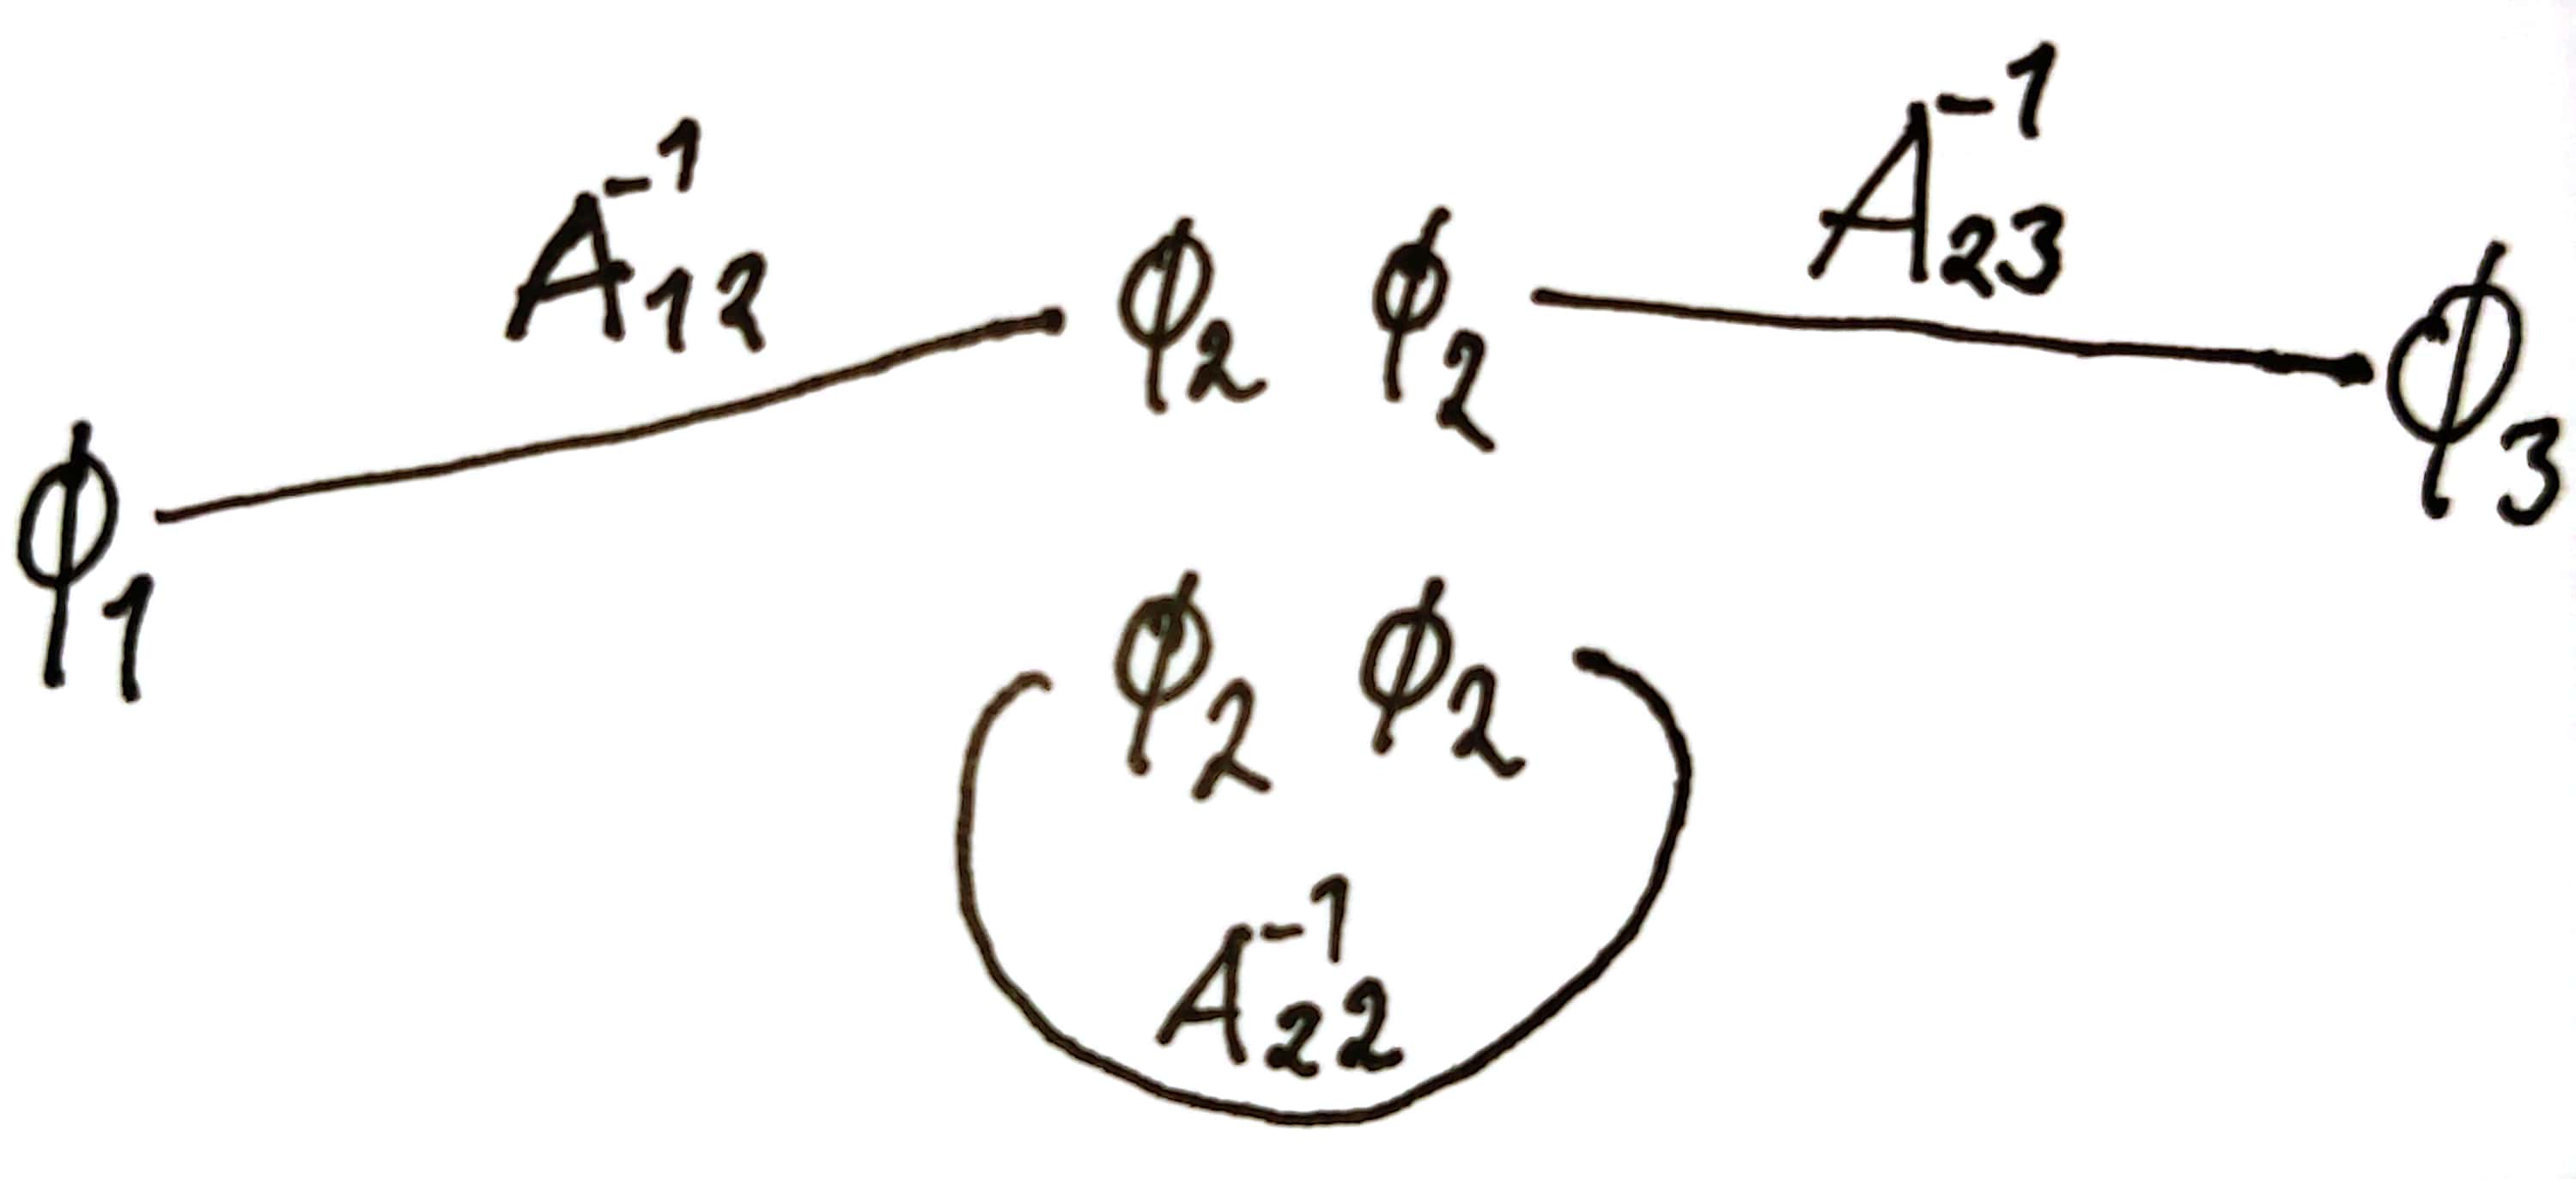
\includegraphics[width=.3\textwidth]{fig/pathint_01.jpg} }
    &&+&&
    \parbox{.3\textwidth}{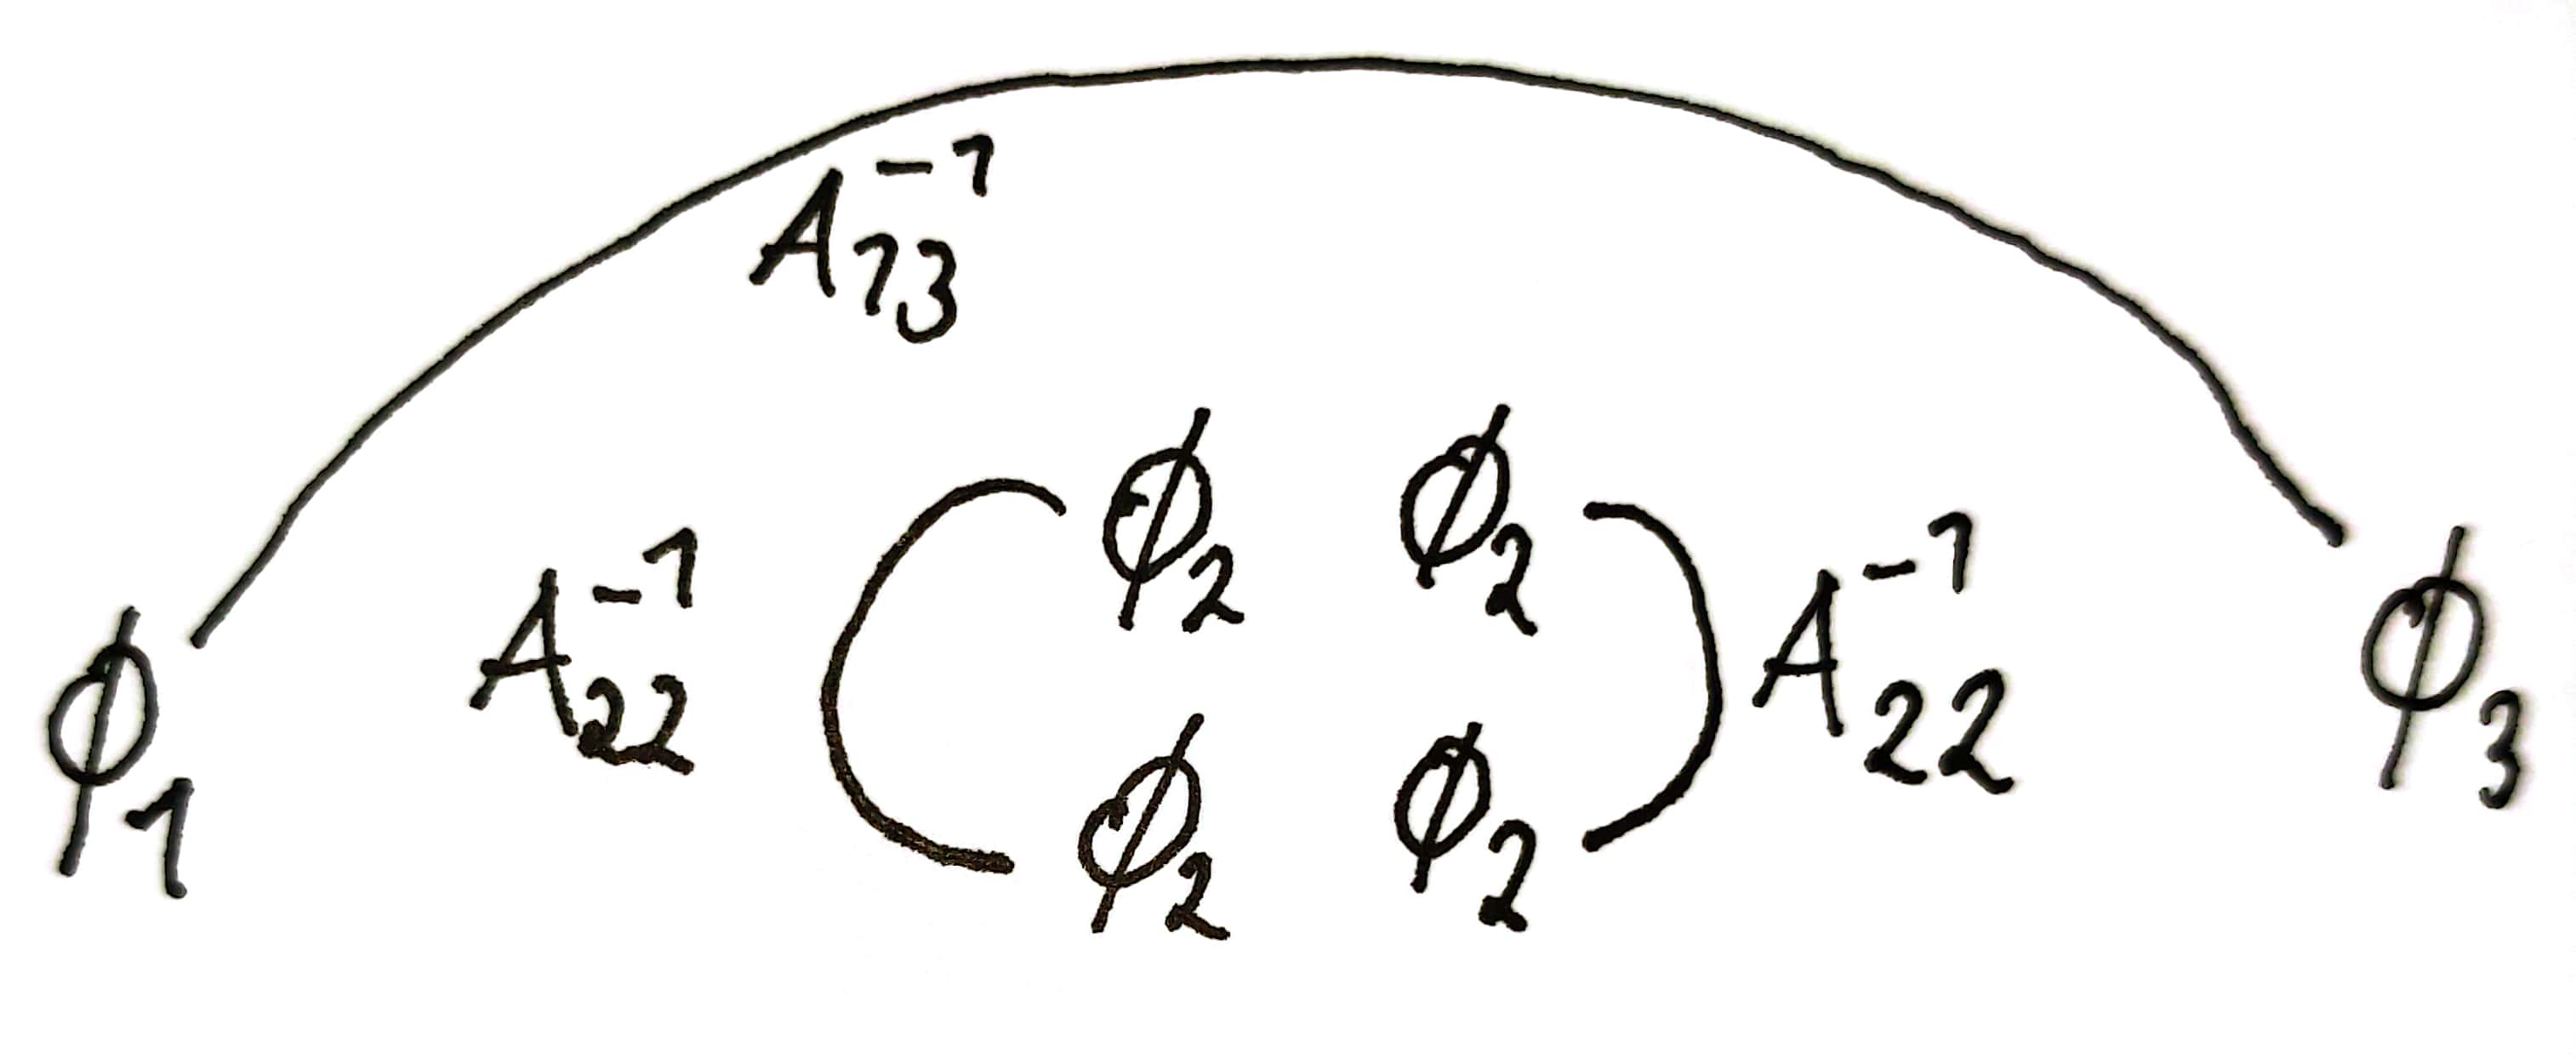
\includegraphics[width=.3\textwidth]{fig/pathint_02.jpg} }\\
    &= &&
    s_1 A_{12}^{-1} A_{22}^{-1} A_{23}^{-1}
    &&+&&s_2 A_{13}^{-1} \left( A_{22}^{-1} \right)^2.
\end{align}
%
Here, $s_1$ and $s_2$ are \emph{symmetry factors}, which count the number of distinct ways we could have created the same diagrams by connecting propagators.
For the first diagram, $\phi_1$ can be connected 4 ways into the cluster, the cluster can self-connect in three different ways, and we are then left with only one way to connect the cluster to $\phi_3$, so $s_1 = 4 \times 3 \times 1 = 12$.
For the second diagram, there is only one way to connect $\phi_1$ and $\phi_3$, then the first connection in the cluster can be done in $3$ ways, and the second is then forced.
This gives $s_2 = 3$.

Feynman diagrams often appear in a more abstract form, where the fields and propagators are implied.
The diagrams illustrated above are then
%
\begin{align}
    \E{\phi_1 \phi_2^4 \phi_3} = 
    \parbox{16mm}{
    \centering
    \begin{fmfgraph*}(16,10)
        \setval
        \fmfleft{i}
        \fmfright{o}
        \fmftop{t}
        \fmf{plain}{i,c,o}
        \fmffreeze
        \fmf{plain,left}{c,t}
        \fmf{plain,left}{t,c}
    \end{fmfgraph*}
    }
    +
    \parbox{16mm}{
    \centering
    \begin{fmfgraph*}(10,4)
        \setval
        \fmfleft{i}
        \fmfright{o}
        \fmf{plain,left}{i,c,o,c,i}
    \end{fmfgraph*}\\
    \begin{fmfgraph*}(16,2)
        \setval
        \fmfleft{i}
        \fmfright{o}
        \fmf{plain}{i,c,o}
    \end{fmfgraph*}
    }
    .
\end{align}
%
Computation of Feynman diagrams is one of the main tasks in perturbative field-theory.
However, the difficulty comes when the ``vertices'', such as $\phi_2^4$ are not just a single index, but a sum over indices, so $\sum_\alpha \phi_\alpha^4$.
The resulting propagators are then summed over matching indices, and in the continuum limit, these sums becomes integrals.
Integrals are, as we all know, not easy to solve, so this is the main challenge of perturbative calculations.

\begin{framed}\noindent
    \textit{Exercise}:
    Draw all diagrams, and count the symmetry factor for the following two expectation values:
    %
    \begin{align}
        \E{\phi_1\phi_2^3\phi_3^3\phi_4} & = 
        \parbox{16mm}{
        \centering
        \begin{fmfgraph*}(16,10)
            \setval
            \fmfleft{i}
            \fmfright{o}
            \fmf{plain}{i,c1}
            \fmf{plain,left,tension=1/2}{c1,c2,c1}
            \fmf{plain}{c2,o}
        \end{fmfgraph*}
        }
        +  \cdots\\
        \E{\phi_1\phi_2^4\phi_3^4\phi_4} & = 
        \parbox{16mm}{
        \centering
        \begin{fmfgraph*}(16,10)
            \setval
            \fmfleft{i}
            \fmfright{o}
            \fmf{plain}{i,c1}
            \fmf{plain}{c2,o}
            \fmf{plain,tension=1/3}{c1,c2}
            \fmf{plain,left,tension=1/3}{c1,c2,c1}
        \end{fmfgraph*}
        }
         +  \cdots
    \end{align}
    %
    The two diagrams we included here are so-called \emph{self-energy} diagrams, one of the most common types of diagrams.
    In fact, the second diagram has several names, for example ``sunset diagram'' or ``Jupiter diagram''.
    It is ubiquitous, as it appears in ``$\phi^4$'' theories, one of the true work-horses of theoretical physics.
\end{framed}

